\section{Storage Hierarchy}

\subsection{Expanding on von Neumann Architecture} 

  So far, our model of the computer has been a simple von Neumann architecture which consists of a CPU and memory. However, there are many other intricacies that are extremely important in practice, and we'll expand on each one by one. 
  
  \begin{definition}[Computer Architecture]
    In our elaborated computer architecture, a computer consists of the components. 
    \begin{enumerate}
      \item A \textbf{CPU} that consists of an arithmetic logic unit (ALU), registers, and a \textbf{bus interface} that controls the input and output. 
      \item The \textbf{IO bridge} that handles communication between everything. 
      \item The \textbf{system bus} that connects the CPU to the IO bridge. 
      \item The \textbf{memory bus} that connects the memory to the IO bridge. 
      \item The \textbf{IO bus} that connects the IO devices and disk to the IO bridge. 
      \item \textbf{IO devices} like mouse, keyboard, and monitor. 
      \item The \textbf{disk controller and disk} that stores data. 
    \end{enumerate} 
    \begin{figure}[H]
      \centering 
      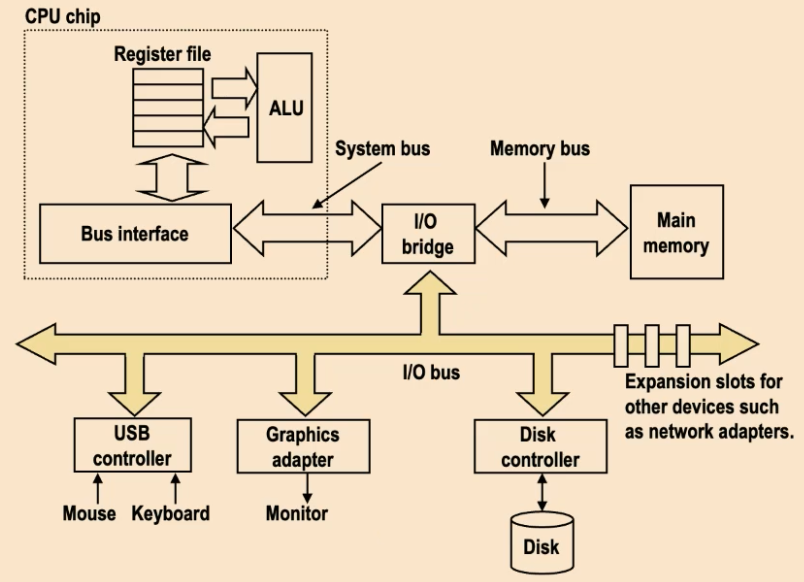
\includegraphics[scale=0.4]{img/io.png}
      \caption{Diagram of the IO bus.} 
      \label{fig:io}
    \end{figure}
  \end{definition}

  We can see from the diagram above that the CPU can directly access registers (since it's in the CPU itself) and the main memory (since it's connected to the memory bus). However, to access something like the disk, it must go through the disk controller. This gives us our first categorization of memory. 

  \begin{definition}[Primary Storage]
    \textbf{Primary storage devices} are directly accessible by the CPU and are used to store data that is currently being processed. This includes CPU registers, cache memory, and RAM. In memory, the basic storage unit is normally a \textbf{cell} (one bit per cell), which is the physical material that holds information. A \textbf{supercell} has address and data widths (number of bits), which is analogous to a lock number and the lock capacity, respectively. It is called random access since it takes approximately the same amount of time to access any cell in memory. There are two primary ways that this is implemented:  
    \begin{enumerate}
      \item \textbf{Static RAM (SRAM)} stores data in small electrical circuits (e.g. latches) and is typically the fastest type of memory. However, it is more expensive to build, consumers more power, and occupies more space, limiting the SRAM storage. 
      \item \textbf{Dynamic RAM (DRAM)} stores data using electrical components (e.g. capacitors) that hold an electrical charge. It is called \textit{dynamic} because a DRAM system must frequently refresh the charge of its capacitors to maintain a stored value. It also requires error correction which introduces redundancy. 
    \end{enumerate}

    \begin{table}[H]
      \centering
      \begin{tabular}{|l|l|l|l|}
      \hline
      \textbf{Device} & \textbf{Capacity} & \textbf{Approx. latency} & \textbf{RAM type} \\ \hline
      Register & 4 - 8 bytes & < 1 ns & SRAM \\ \hline
      CPU cache & 1 - 32 megabytes & 5 ns & SRAM \\ \hline
      Main memory & 4 - 64 gigabytes & 100 ns & DRAM \\ \hline
      \end{tabular}
      \caption{Memory hierarchy characteristics}
      \label{tab:memory_hierarchy}
    \end{table}
  \end{definition}

  \begin{definition}[Secondary Storage]
    \textbf{Secondary storage devices} are not directly accessible by the CPU and are used to store data that is not currently being processed. This includes hard drives, SSDs, and magnetic tapes. There are two primary ways: 
    \begin{enumerate}
      \item \textbf{Spinning disks} store data on a magnetic surface that spins at high speeds.
      \item \textbf{Solid state drives (SSDs)} store data on flash memory chips.
    \end{enumerate}
  \end{definition}

  There are three key components of memory that we should think about: 
  \begin{enumerate}
    \item The \textbf{capacity}, i.e. amount of data, it can store (how large the water tank is). 
    \item The \textbf{latency}, i.e. amount of time it takes for a device to respond with data after it has been instructed to perform a data retrieval operation (how fast the data flows). 
    \item The \textbf{transfer rate} or \textbf{thoroughput}, i.e. amount of data that can be moved between the device and main memory (how wide the pipe is). Naively, with one channel and sequential transfer the transfer rate is one over the latency. 
  \end{enumerate}

  We must provide a good balance of these three qualities, and also note that there are some physical limitations (i.e. latency cannot be faster than speed of light), and this is more effectively done through a hierarchical memory system.

  \begin{figure}[H]
    \centering 
    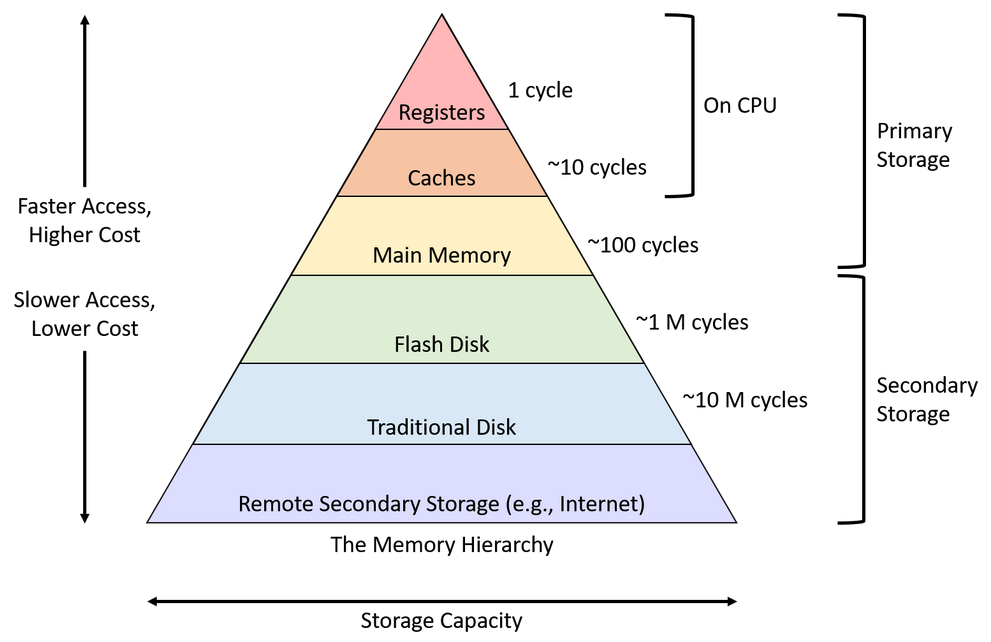
\includegraphics[scale=0.4]{img/memory_hierarchy.png}
    \caption{Memory hierarchy.} 
    \label{fig:memory_hierarchy}
  \end{figure}

  For example when we want to read from the disk, the CPU must request to the bus interface, which travels through the bus interface, I/O bridge, I/O bus, disk controller, and to the disk itself. Then the data goes back through the disk controller, I/O bus, I/O bridge, through the memory bus, and resides in the main memory. Note that disks are block addressed, so it will transfer the entire block of data into the memory. It must specify a \textbf{destination memory address (DMA)}. When the DMA completes, the disk controller notifies the CPU with an \textit{interrupt} (i.e. asserts a special interrupt pin on the CPU), letting it know that the operation has finished. This signal goes through the disk controller to the IO bridge to the CPU. From now on, the CPU knows that there is memory that it can access to run an application loaded in memory. 

\subsection{Disk} 

  \begin{definition}[Hard Disk Drives]
    Back then, there were \textbf{hard disk drives (HDDs)} that literally had a spinning wheel and a needle head that read the data. 
    \begin{figure}[H]
      \centering 
      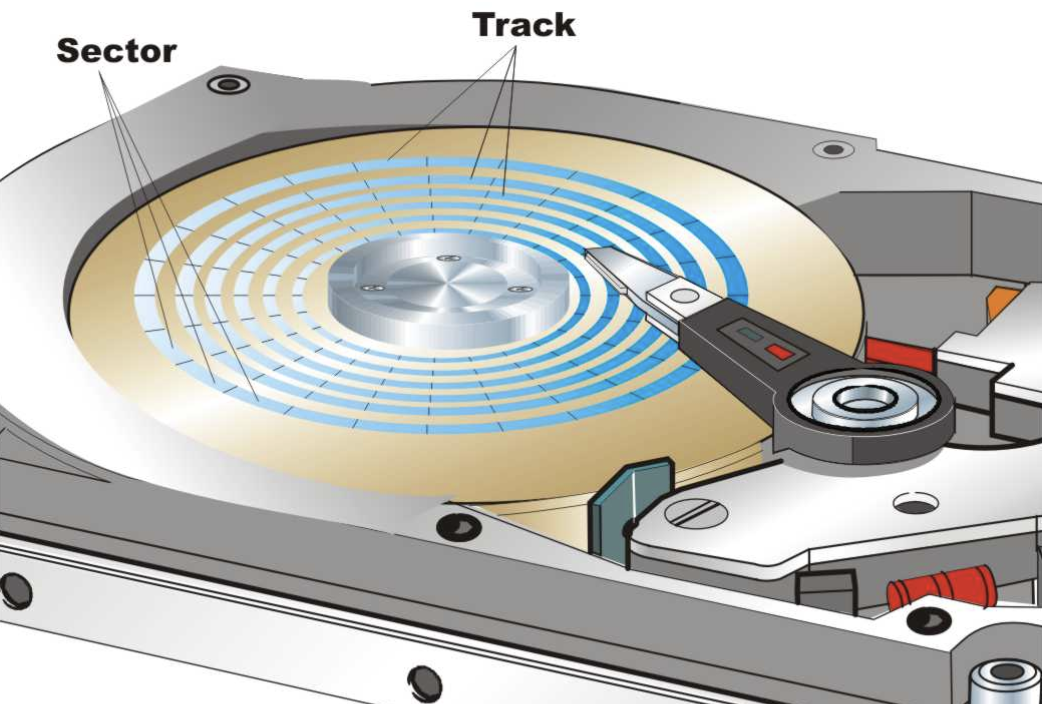
\includegraphics[scale=0.4]{img/hdd.png}
      \caption{Visual diagram of hard disk drive with its sectors. } 
      \label{fig:hdd}
    \end{figure}
    \begin{enumerate}
      \item HDDs are not random access since the data must be sequentially read. This was disadvantageous since the spinning wheel had to spin to the correct location, which took time. The needle also had to move to the correct location, which also took time and therefore read and write speeds were dominated by the time it took to move the needle.
      \item The smallest unit of data that can be read is a complete disk sector (not a single byte like RAM). 
    \end{enumerate}
  \end{definition}

  \begin{definition}[Solid State Drives]
    Now, we have \textbf{solid state drives (SSDs)} that store data on flash memory chips. This is advantageous since there are no moving parts, so the latency is much lower and the latency is not dominated by the time it takes to move the needle. 
    \begin{enumerate}
      \item SSDs are random access. 
      \item The smallest unit of data is a \textbf{page}, which is usually 4KB and maybe for high scale computers 2-4 MB (but on ``Big Data'' applications big but computers, it can be up to 1GB). 
      \item A collection of pages, usually 128 pages, is called a \textbf{block}, making is 512KB. 
    \end{enumerate}
  \end{definition}

  While virtually all RAM and primary storage devices are \textbf{byte addressable} (i.e. you can access any byte in memory), secondary storage devices are \textbf{block addressable} (i.e. you can only access a block of memory at a time). Therefore, to access a single byte in secondary storage, you must first load the entire block into memory, calculate which byte from that block you want, and then access it. Therefore, you need both the block number $x$ and the offset $o$ to access a byte in secondary storage, which is why it is even slower than accessing RAM. 

  \begin{figure}[H]
    \centering 
    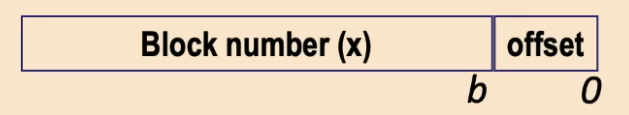
\includegraphics[scale=0.4]{img/block_offset.png}
    \caption{Block offset.} 
    \label{fig:block_offset}
  \end{figure}

  Therefore, you can think of raw data in units of blocks of size $2^b$ for some $b$ bits. 
  \begin{enumerate}
    \item Take the low order $b$ bits of a byte address as an integer, which is the offset of the addressed byte in the block. 
    \item THe rest of the bits are the block number $x$, which is an unsigned long. 
    \item You request the block number $x$, receive the block contents, and then extract the requested byte at offset in $x$ i.e. calculate \texttt{block[x][offset]}. 
  \end{enumerate}

\subsection{Locality}

  So far, we have abstracted away most of these memory types as a single entity with nearly instantaneous access, but in practice this is not the case. The most simple way is to simply have RAM and our CPU registers, but by introducing more intermediate memory types, we can achieve greater efficiency. 

  \begin{definition}[Locality]
    \textbf{Locality} is a principle that generally states that a program that accesses a memory location $n$ at time $t$ is likely to access memory location $n + \epsilon$ at time $t + \epsilon$. This principle motivates the design of efficient caches. 
    \begin{enumerate}
      \item \textbf{Temporal locality} is the idea that if you access a memory location, you are likely to access it again soon. 
      \item \textbf{Spatial locality} is the idea that if you access a memory location, you are likely to access nearby memory locations soon.
    \end{enumerate}
    This generally means that if you access some sort of memory, the values around that address is also likely to be accessed and therefore it is wise to store it closer to your CPU. In CPUs, both the instructions and the data are stored in the cache, which exploits both kinds of locality (repeated operations for temporal and nearby data for spatial). 
  \end{definition}

  \begin{example}[Locality]
    Consider the following code. 
    \begin{lstlisting}
      int sum_array(int *array, int len) {
        int i;
        int sum = 0;

        for (i = 0; i < len; i++) {
          sum += array[i];
        }

        return sum;
      }
    \end{lstlisting}
    \begin{enumerate}
      \item \textbf{Temporal Locality}
        \begin{enumerate}
          \item We cycle through each loop repeatedly with the same add operation, exploiting temporal locality.  
          \item The CPU accesses the same memory (stored in variables \texttt{i}, \texttt{len}, \texttt{sum}, \texttt{array}) within each iteration and therefore at similar times. 
        \end{enumerate}
      \item \textbf{Spatial Locality}
        \begin{enumerate}
          \item The spatial locality is exploited when the CPU accesses memory locations from each element of the array, which are contiguous in memory. 
          \item Even though the program accesses each array element only once, a modern system loads more than one \texttt{int} at a time from memory to the CPU cache. That is, accessing the first array index fills the cache with not only the first integer but also the next few integers after it too. Exactly how many additional integers get moved depends on the cache's \textbf{block size}. For example, a cache with a 16 byte block size will store \texttt{array[i]} and the elements in \texttt{i+1}, \texttt{i+2}, \texttt{i+3}. 
        \end{enumerate}
    \end{enumerate}
  \end{example}

  We can see the differences in spatial locality in the following example. 

  \begin{example}
    One may find that simply changing the order of loops can cause a significant speed up in your program. Consider the following code. 
    \begin{figure}[H]
      \centering 
      \noindent\begin{minipage}{.5\textwidth}
      \begin{lstlisting}[]{Code}
        float averageMat_v1(int **mat, int n) {
          int i, j, total = 0;

          for (i = 0; i < n; i++) {
            for (j = 0; j < n; j++) {
              // Note indexing: [i][j]
              total += mat[i][j];
            }
          }
          return (float) total / (n * n);
        }
      \end{lstlisting}
      \end{minipage}
      \hfill
      \begin{minipage}{.49\textwidth}
      \begin{lstlisting}[]{Output}
        float averageMat_v2(int **mat, int n) {
          int i, j, total = 0;

          for (j = 0; j < n; j++) {
            for (i = 0; i < n; i++) {
              total += mat[i][j];
            }
          }
          return (float) total / (n * n);
        }
        .
      \end{lstlisting}
      \end{minipage}
      \caption{Two implementations of taking the total sum of all elements in a matrix.} 
      \label{fig:matrix_sum}
    \end{figure}
    It turns out that the left hand side of the code executes about 5 times faster than the second version. Consider why. When we iterate through the \texttt{i} first and then the \texttt{j}, we access the values \texttt{array[i][j]} and then by spatial locality, the next few values in the array, which are \texttt{array[i][j+1]}, ... are stored in the cache. 
    \begin{enumerate}
      \item In the left hand side of the code, these next stored values are exactly what is being accessed, and the CPU can access them in the cache rather than having to go into memory. 
      \item In the right hand side of the code, these next values are \textit{not} being accessed since we want to access \texttt{array[i+1][j]}, .... Unfortunately, this is not stored in the cache and so for every $n^2$ loops we have to go back to the memory to retrieve it. 
    \end{enumerate}
  \end{example}

\subsection{Caches}

    In theory, a cache should know which subsets of a program's memory it should hold, when it should copy a subset of a program's data from main memory to the cache (or vice versa), and how it can determine whether a program's data is present in the cache. Let's talk about the third point first. It all starts off with a CPU requesting some memory address, and we want to determine whether it is in the cache or not. To do this, we need to look a little deeper into memory addresses. 

    \begin{definition}[Portions of Memory Addresses]
      A memory address is a $m$-bit number.\footnote{64 in 64-bit machines.} It is divided up into three portions. 
      \begin{enumerate}
        \item The \textbf{tag} field with $t$ bits at the beginning.
        \item The \textbf{index} field with $i$ bits in the middle. 
        \item The \textbf{offset} field with $o$ bits at the end.
      \end{enumerate}
      The tag plus the index together refers to the \textbf{block number}. 
      \begin{figure}[H]
        \centering 
        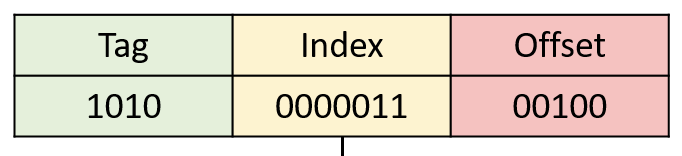
\includegraphics[scale=0.4]{img/memory_portions.png}
        \caption{Portions of a 16 bit memory address with $t = 4, i = 7, o = 5$. } 
        \label{fig:memory_portions}
      \end{figure}
    \end{definition}

    Before we see why we do this, we should also define the portions of a CPU. 

    \begin{definition}[CPU Cache]
      A \textbf{CPU cache} divides its storage space as follows. A cache is essentially an array of sets, where $S$ is the number of sets. Each set is divided into $E$ units called \textbf{cache lines/rows}, with each cache line independent of all others and contains two important types of information. 
      \begin{enumerate}
        \item The \textbf{cache block} stores a subset of program data from main memory, of size $2^o$.\footnote{In Intel computers, it is typically 64 bytes long and for Mac Silicon, it is 128 bytes.} Sometimes, the block is referred to as the cache line. Note that is the cache block size is $2^o$ bytes, then the block offset field has length $\log_2 2^o = o$.
        \item The \textbf{metadata} stores the \textbf{valid bit} (which tells us if the actual data in memory is valid), and the \textbf{tag} of length $t$ (the same as the tag length of the memory address) which tells us the memory address of the data in the cache. 
      \end{enumerate}
      Therefore, the \textbf{cache size} is defined to be $C = S \cdot E \cdot B$ (the metadata is not included). 
      \begin{figure}[H]
        \centering 
        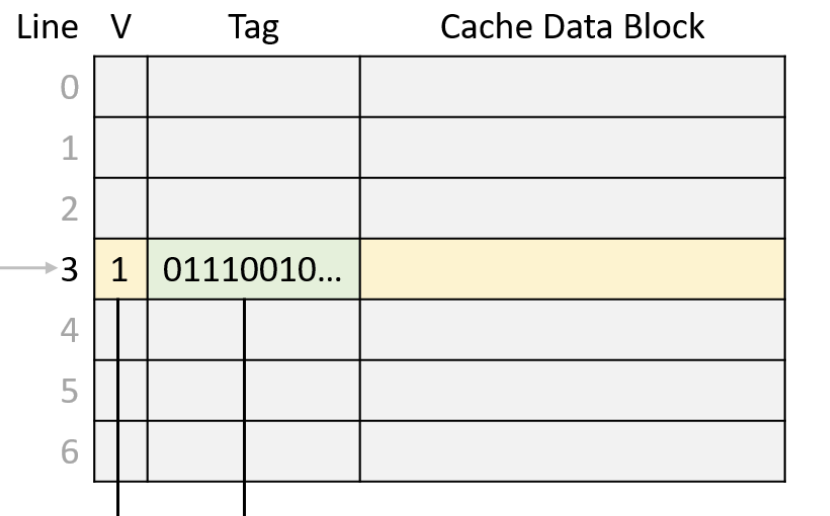
\includegraphics[scale=0.4]{img/direct_mapped_cache.png}
        \caption{Diagram of a direct-mapped cache.} 
        \label{fig:direct_mapped_cache}
      \end{figure}
      CPU caches are built-in fast memory (SRAM) that stores stuff. There are two types: 
      \begin{enumerate}
        \item \textbf{i-cache} stores copies of instructions. 
        \item \textbf{d-cache} stores copies of data from commonly referenced locations. 
      \end{enumerate}
      We saw that caches come in different levels, they all just hold words retrieved from a higher level of memory. 
      \begin{enumerate}
        \item CPU registers hold words retrieved from L1 cache. 
        \item L1 holds cache lines retrieved from L2 cache. 
        \item L2 cache holds cache lines retrieved from L3 cache or the main memory.  
        \item Main memory holds disk blocks retrieved from local disks. 
        \item Local disks hold blocks retrieved from remote disks or network servers. 
      \end{enumerate}

      \begin{figure}[H]
        \centering 
        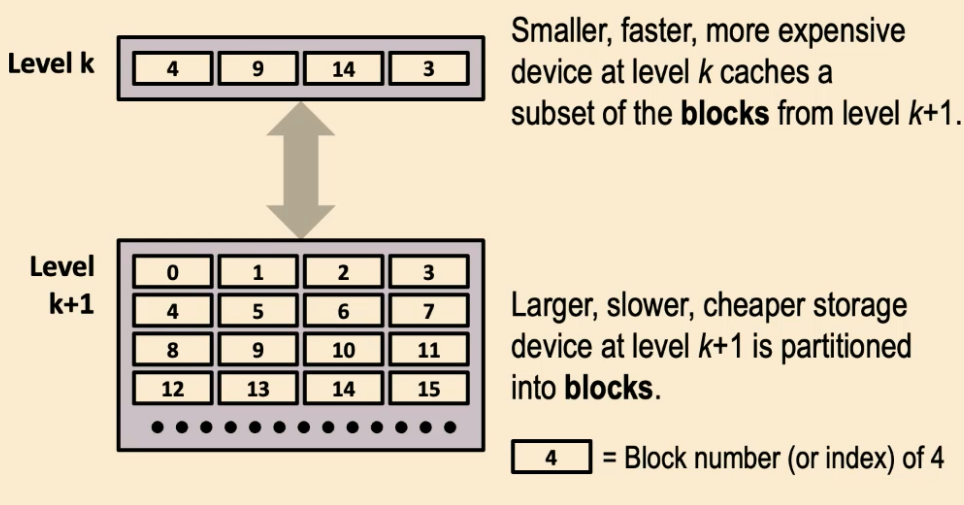
\includegraphics[scale=0.4]{img/cache_retrieve.png}
        \caption{How caches retrieve data from higher levels of memory.} 
        \label{fig:cache_retrieve}
      \end{figure}
    \end{definition}

    \begin{example}[Simple Calculations]
      Given a direct-mapped cache specified by a block size of 8 bytes and a cache capacity of 4 KB, 
      \begin{enumerate}
        \item the cache can hold 512 blocks. 
        \item the block offset field is $\log_2 8 = 3$ bits wide. 
        \item the address \texttt{0x1F = 0b00011111} is in block number $3$ since the last three bits are the offset, and whatever is left (passed through the hashamp, which is simply modulo), is the block number. 
      \end{enumerate}
    \end{example}

    In \textbf{I/O caches}, software keeps copies of cached items in memory, indexed by name via a hash table.

    At the lowest level, registers are explicitly program-controlled, but when accessing any sort of higher memory, the CPU doesn't know whether some data is in the cache, memory, or the disk. 

    \begin{figure}[H]
      \centering 
      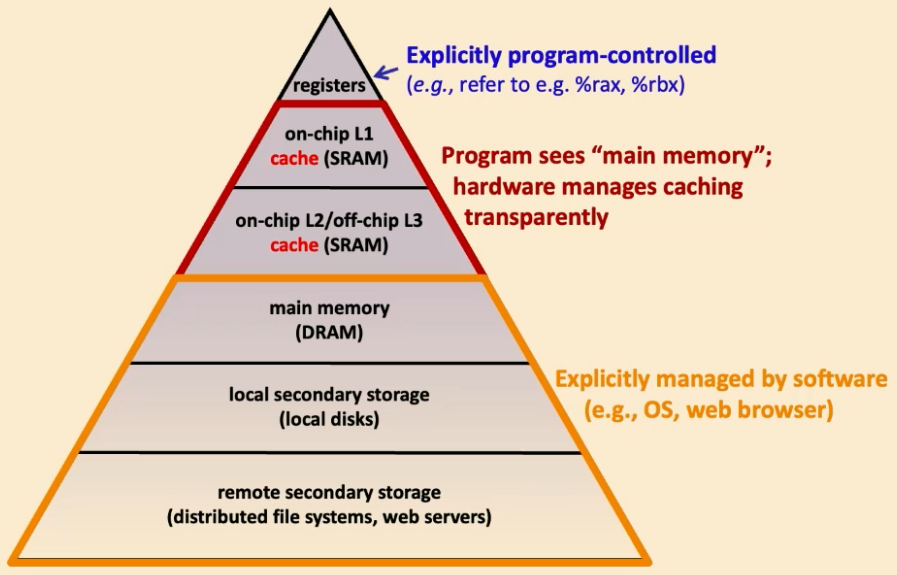
\includegraphics[scale=0.4]{img/hierarchy2.png}
      \caption{} 
      \label{fig:hierarchy2}
    \end{figure}

    Finally, let's compare software vs hardware caches. 

    \begin{definition}[Software Caches]
      When implementing caches in software, there are large time differences (DRAM vs disk, local vs remote), and they can be tailored to specific uses cases. They also have flexible and sophisticated approaches with data structures (like trees) and can perform complex computation. 
    \end{definition}

    Theoretically, when implementing hash tables, you never actually have to evict something. You can have the values of the table to be a linked list where we add to the head. If there is unlimited chaining, we have a full associative cache, and if we have limited chaining (e.g. 5), it is like a 5-way set associative cache. If it goes out of bound, we can implement LRU by removing the tail of the linked list. 

    \begin{definition}[Hardware Caches]
      In hardware caches, there are smaller time differences, needs to be as fast as possible, and parallelization is emphasized. 
    \end{definition}

    There are slightly different implementations of caching, and for each implementation, we will describe 
    \begin{enumerate}
      \item how to load data from memory into the cache, 
      \item how to retrieve data from the cache, 
      \item how to write data to the cache. 
    \end{enumerate}

  \subsubsection{Direct Mapped Cache} 

    A direct mapped cache is a caching implementation when we assume that $E = 1$, which means that for any given memory address, there is only one possible cache line that can store this data at that memory address. That is, the cache is really just a bunch of sets with one cache line each, and each cache line is completely isolated from the others. Whether we load data from memory into cache or try to retrieve data from the cache, it's really the same process. 

    \begin{theorem}[Placement]
      To load data from memory into the cache, which happens when there is a \textbf{cache miss}, we do the following. 
      \begin{enumerate}
        \item The CPU requests a memory address $M = (T, I, O)$. 
        \item There exists a hashmap $H$ that maps the index $I$ to a cache line. 
        \item At line $H(I)$, we can get a cache miss and must load from memory into this cache. 
        \item We wait until the memory has retrieved the data from the portion of the memory. i.e. we wait for the $2^o$ bytes located at addresses $(T, I, 0\ldots 0)$ to $(T, I, 1\ldots 1)$. Call this data $D$. 
        \item The $2^o$ byte string $D$ is stored in the cache data block at line $M(I)$,ready to be used. 
      \end{enumerate}
    \end{theorem}

    \begin{theorem}[Lookup]
      To see whether a requested memory address is in the cache, we do the following. 
      \begin{enumerate}
        \item The CPU requests a memory address $M = (T, I, O)$. 
        \item There exists a hashmap $H$ that maps the index $I$ to a cache line. 
        \item At line $H(I)$, check the cache line's valid bit. If it is not valid, then this is a cache miss and we must go to the memory to retrieve the data, leading to the above process. 
        \item Since there could be multiple $I$ that maps to the same cache line, there will be overlap. But this is where the tag portion comes in. At cache line $H(I)$, the CPU checks the cache tag to see if it matches the memory tag $T$. 
        \item If it does, then we have just found a way to identify the first $t + i$ bits of the requested memory address, and we have gotten a cache hit. Now, we know that the cache's data block holds the data that the program is looking for. We use the low-order offset bits of the address to extract the program's desired data from the stored block. 
      \end{enumerate}
      \begin{figure}[H]
        \centering 
        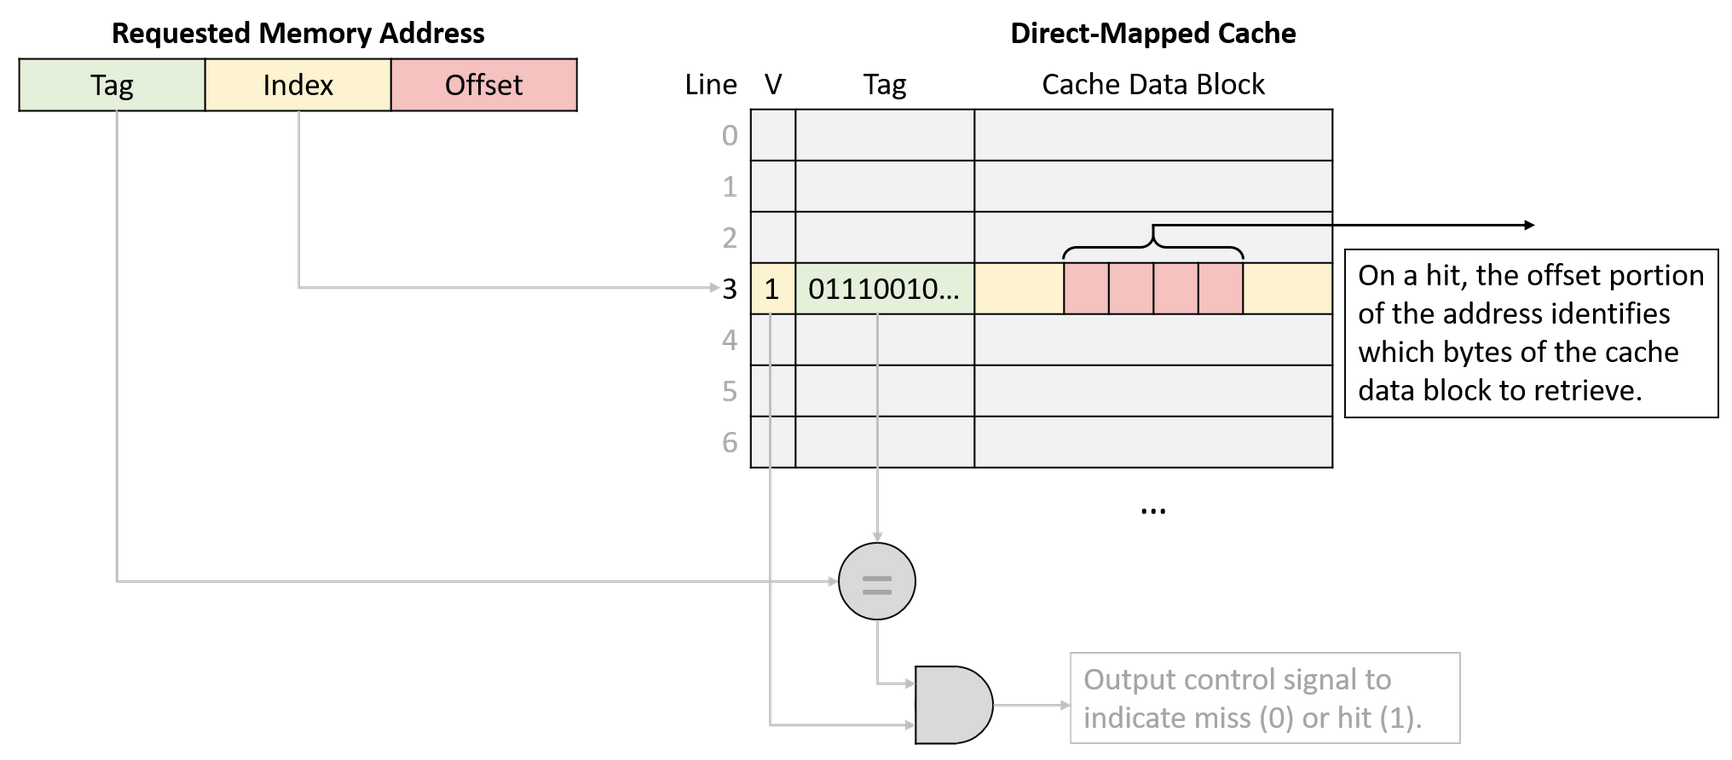
\includegraphics[scale=0.4]{img/cache_request.png}
        \caption{Diagram of a cache request. Note that since the entire data in the memory block stored in the cache, we can take advantage of spatial locality.}  
        \label{fig:cache_request}
      \end{figure}
    \end{theorem}

    So far, we've talked about reading operations, but what about writing to the cache? It is generally implemented in two ways. 

    \begin{definition}[Write-Through, Write-Back Cache]
      Note that when we write data to cache, it does not need to be immediately written to memory, but rather it can be flushed to memory at a later time. This is efficient since if we have repeated operations on a single memory address, we don't have to go back and forth between the CPU and memory. 
      \begin{enumerate}
        \item In a \textbf{write-through cache}, a memory write operation modifies the value in the cache and simultaneously writes the value to the corresponding location in memory. It is always synchronized. 
        \item In a \textbf{write-back cache}, a memory write operation modifies the value stored in the cache's data block, but does \textit{not} update main memory. Instead, the cache sets a \textbf{dirty bit} in the metadata to indicate that the cache block has been modified. The modified block is only written back to memory when the block is replaced in the cache. 

        \begin{figure}[H]
          \centering 
          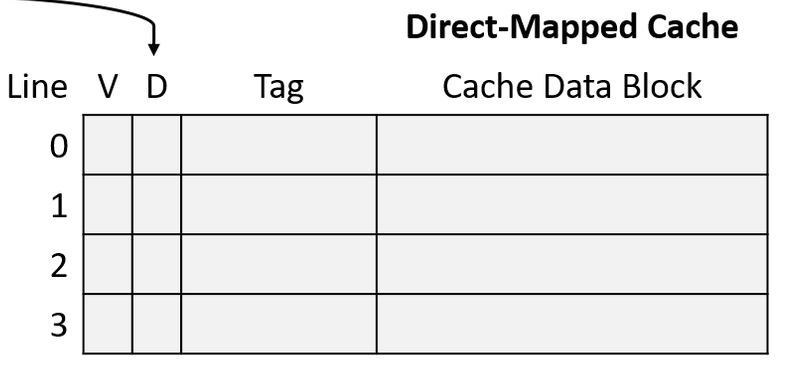
\includegraphics[scale=0.4]{img/dirty_bit.png}
          \caption{A dirty bit is a one bit flag that indicates whether the data stored in a cache line has been modified. When set, the data in the cache line is out o sync with main memory and must be written back (flushed) back to memory before eviction. } 
          \label{fig:dirty_bit}
        \end{figure}
      \end{enumerate}
      As usual, the difference between the designs reveals a trade-off. Write-through caches are less complex than write-back caches, and they avoid storing extra metadata in the form of a dirty bit for each line. On the other hand, write-back caches reduce the cost of repeated writes to the same location in memory.
    \end{definition}

    \begin{theorem}[Replacement]
      Replacement occurs exactly the same way as if we just did a placement and is trivial. We retrieve the data block from the memory and store it in the cache. Direct-mapping conveniently determines which cache line to evict when loading new data. Given new memory $M = (T, I, O)$, you \textit{must} evict the cache line at $H(I)$. 
    \end{theorem}

  \subsubsection{N way Set-Associative Cache}

    Note that for both examples, given a fixed hashmap $H$ it is not possible to store data in two memory addresses $M_1$ and $M_2$ where both $H(I_1) = H(I_2)$. Therefore, the choice of hashing must be done so that it minimizes the number of collisions. So far, we have only considered memory read operations for which a CPU performs lookups on the cache. Caches must also allows programs to store values. However, there is a better way to do this: just construct it so that each set has more than one cache line, and so data in index portions of different memory addresses can be stored in different cache lines.

    In here, we deal with $E \neq 1$, and so there are multiple set each with multiple lines. This means that the cache is more like a 2D array, and when we want to retrieve an index, we must look through the $H(I)$th line in \textit{each} set to see if the tag matches. 

    \begin{theorem}[Lookup]
      To see whether a requested memory address is in the cache, we do the following. 
      \begin{enumerate}
        \item The CPU requests a memory address $M = (T, I, O)$. 
        \item We iterate through each of the $S$ sets in the cache, looking at cache line $M(I)$. 
        \item For each line, we check if it is valid and if so, whether the line tag matches the memory tag. If we get a hit, then we have found the data in the cache. 
      \end{enumerate}

      \begin{figure}[H]
        \centering 
        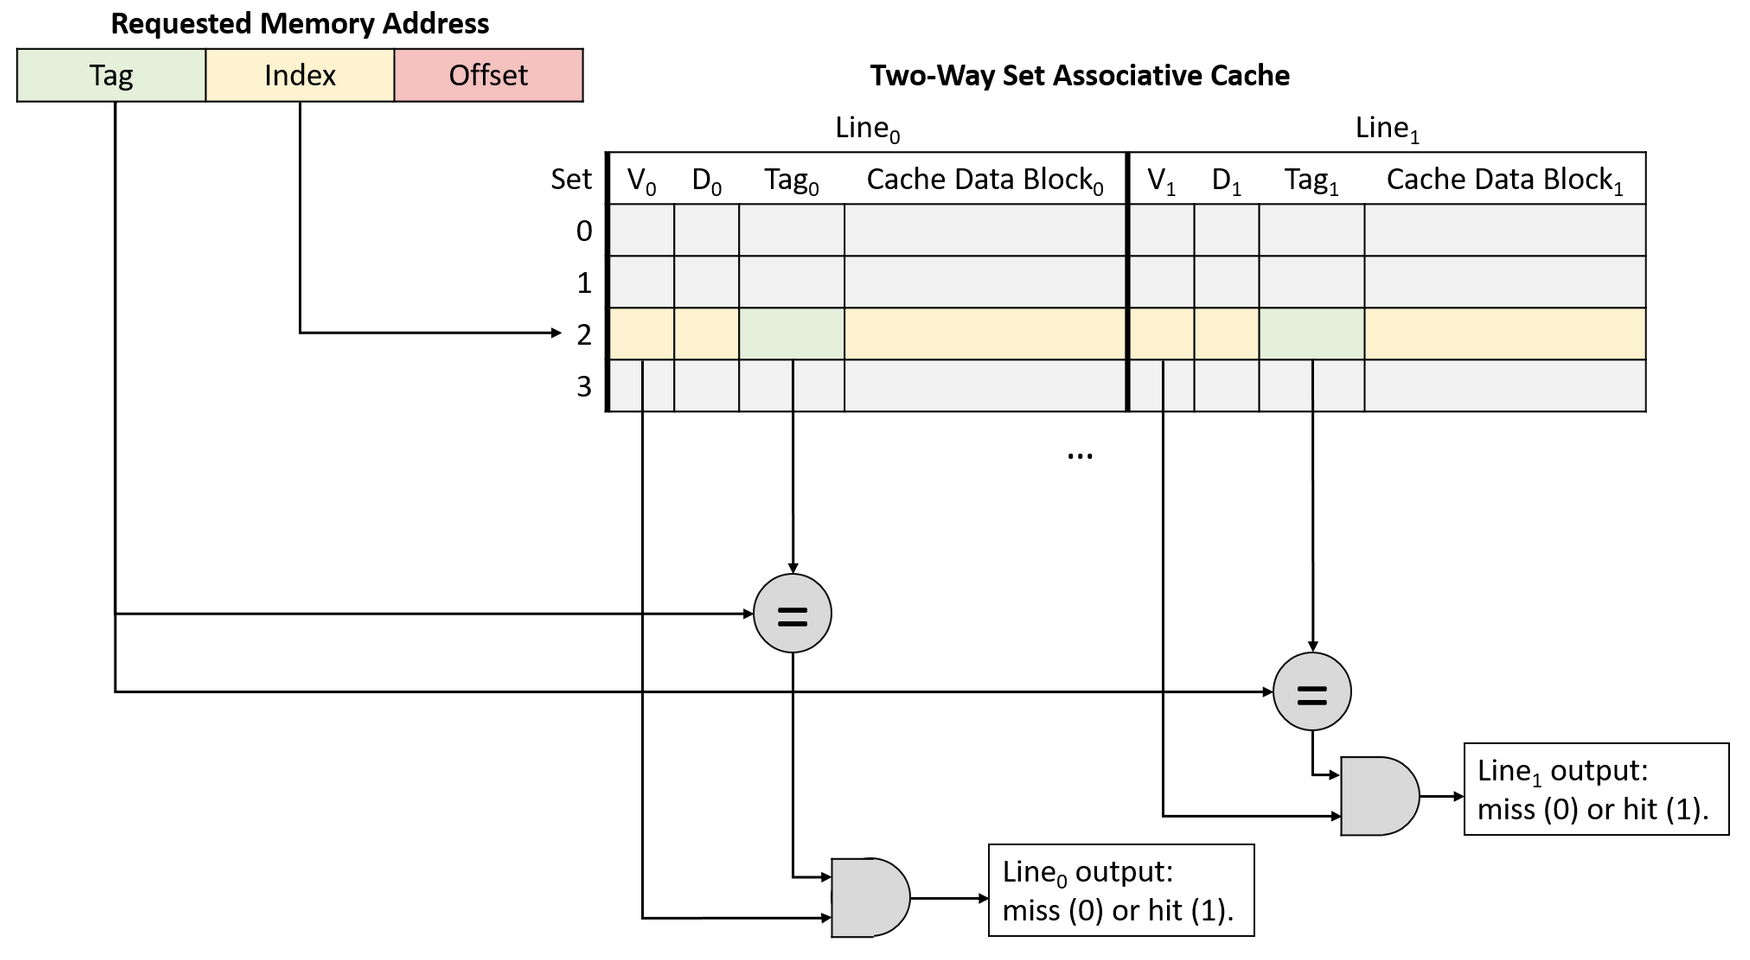
\includegraphics[scale=0.4]{img/retrieve_set_associative.png}
        \caption{Diagram of a 2 set-associative cache.} 
        \label{fig:retrieve_set_associative}
      \end{figure}
    \end{theorem}

    If you have a \textbf{fully associative cache}, then you have one set with $E = C/B$ lines. Therefore, you can really put any memory address data in any cache line. There is a clear tradeoff here. As we increase $N$, we can get more flexibility in using all of our cache space, but the time complexity of retrieving and writing data scales linearly. In fact, this linear scan is too slow for a cache, which is why you need to implement some parallel tag search, but this turns out to be quite expensive to build.\footnote{You have to copy the request tag with a circuit and compare it to all the tags in the cache, which turns out to be a much larger circuit.}
  
    Though we have a more robust implementation with associative mapping, placement and replacement now face the problem of \textit{which} set to place the data in or evict existing data. 

    \begin{theorem}[Placement]
      To load data from memory into the cache this is trivial since we can just go through the sets, find one where the valid bit is $0$, and just place the data there.  
    \end{theorem}

    In replacement, this is a bit trickier, but using the principle of temporal locality, we can try and replace the least recently used cache. This tries to minimize cache misses, but not slow down the lookup too much. 

    \begin{theorem}[Replacement]
      To replace data on the cache, we use the \textbf{least recently used (LRU)} algorithm. This matches temporal locality, but it also requires some additional state to be kept. 
    \end{theorem}

  \subsubsection{Types of Cache Misses} 

    There are three types of cache misses. 

    \begin{definition}[Cold (Compulsory) Miss]
      A \textbf{cold miss} occurs when the cache is empty and the CPU requests a memory address. This is the first time the CPU is requesting this memory address, and so it must go to the memory to retrieve the data.
    \end{definition}
    
    \begin{definition}[Capacity Miss]
      A \textbf{capacity miss} occurs when the cache is full and the CPU requests a memory address that is not in the cache. This is because the cache is full and so the CPU must evict some data to make space for the new data.
    \end{definition}

    \begin{definition}[Conflict Miss]
      A \textbf{conflict miss} occurs from premature eviction of a warm block. 
    \end{definition}

  Valgrind's cachegrind mode. 

